%!TEX root=document.tex

\section{Introduction}
\label{sec:introduction}

 
Data analysts must sift through very large volumes of data 
to identify trends, insights, or anomalies. 
Given the scale of data, and the relative ease and 
intuitiveness of examining data visually,
analysts often use visualizations as a tool to identify
these trends, insights, and anomalies.
However, selecting the ``right'' visualization often 
remains a laborious and time-consuming task. 
We illustrate the data analysis
process and challenges in choosing good visualizations using a few examples.




\subsection*{Motivating Example}
Consider the (fictional) smartphone app analytics team at a company like Apple or Google,
or one of several startups that provides performance analytics for app authors.
This team is tasked with studying the behavior of various apps on the
app store to discover behavior trends for specific classes of apps, e.g.
extremely popular apps, apps that behave badly etc.
Suppose that App-A is a particular app that has been behaving badly and has
received a lot of consumer complaints. 
The app analytics team would like to discover the reason why App-A is
behaving badly in order to provide feedback to the makers of App-A or to pull
the app from the app store.
The typical workflow to analyze App-A would proceed as follows:
(1) An analyst would pose a query to the metrics database to pull all the
metrics for App-A.
For instance, the analyst may issue the following query:
\noindent 
\begin{align*}
& \tt Q \ \ = \ \ SELECT \ * \ FROM \ \  AppMetrics \ \ WHERE  \ Name=``App\text{-}A"
\end{align*}

\noindent Notice that the results for this query may have millions of records
(e.g. a record for each app session) each with several dozen attributes (e.g.
network usage, power consumption, load time etc).
Thus, directly perusing the query result is simply infeasible.
(2) Next, the analyst studies various properties of the selected metrics by
aggregating the data along different dimensions and measures. 
In this particular scenario, the analyst may want to examine the average power
consumption by device, total crashes grouped by session time, or average load
times by carrier.
To construct these queries, the analyst uses operations such as binning,
grouping, and aggregation.  Frequently, he will generate visualizations to view
the results of the data.
For example, to generate extract the for average load times by carrier, the
analyst would group metrics based on the carrier and then average the app load
times per carrier.
This operation can easily be expressed as the familiar aggregation over group-by
query:
\noindent
\begin{align*}
& \tt Q' = SELECT \ \ carrier,\ AVG(load\_time) \ \ FROM \ \  AppMetrics \\
& \tt \hspace{20pt} WHERE\ Name=``App\text{-}A" \ \ GROUP  \ \ BY \ \ carrier
\end{align*}
The result of the above query is a two-column table that can then be visualized
as a bar-chart. Table \ref{tab:staplerX} and Figure
\ref{fig:staplerX} respectively show an example of the results of this query and
the associated visualization.

%Consider a dataset containing sales records for a nation-wide
%chain of stores.
%Let's say the store's data analyst is interested
%in examining how the newly-introduced heating device, the ``Laserwave
%Oven'', has been doing over the past year.
%The results of this analysis will inform business decisions
%for the chain, including marketing strategies, and the introduction of a
% similar ``Saberwave Oven''.

%The analysis workflow proceeds as follows:
%(1) The analyst poses a query to select the subset of data that she is
%interested in exploring.
%For instance, for the example above, she may issue the query:
%\noindent $${\tt \ Q \ \ = \ \ SELECT \ * \ FROM \ \  Sales \ \ WHERE \ \
%Product=``Laserwave''} $$ 
% \noindent Notice that the results for this query may
% have (say) several million records each with several dozen attributes.
% Thus, directly perusing the query result is simply infeasible.
% (2) Next, the analyst studies various properties of the selected data by
% constructing diverse views or visualizations from the data. In this particular
% scenario, the analyst may want to study total sales by store, quantity in stock
% by region, or average profits by month. To construct these views, the analyst
% can use operations such as binning, grouping, and aggregation, and then generate
% visualizations from the view. For example, to generate the view `total sales by
% store', the analyst would group each sales record based on the store where the
% sale took place and sum up the sale amounts per store. This operation can easily
% be expressed as the familiar aggregation over group-by query:
% \noindent
% \begin{align*}
% & \tt Q' = SELECT \ \ store,\ SUM(amount) \ \ FROM \ \  Sales \ \ WHERE \\
% & \tt Product=``Laserwave" \ \ GROUP  \ \ BY \ \ store
% \end{align*}
% The result of the above query is a two-column table that can then be visualized
% as a bar-chart. Table \ref{tab:staplerX} and Figure
% \ref{fig:staplerX} respectively show an example of the results of this view and
% the associated visualization.

\begin{figure}[h]
	\centering
	\begin{subfigure}{0.49\linewidth}
	   \begin{tabular}{cc} \hline
		  Carrier & Load Times (ms) \\ \hline
		  AT\&T & 180.55 \\ \hline
		  Verizon &  145.50\\ \hline
		  T-Mobile & 122.00 \\ \hline
		  Metro & 90.13 \\ \hline
		  \end{tabular}
		  \caption{tab:staplerX}
		  \caption{Data: Average Load Times by Carrier for App-A}
	\end{subfigure}
	\begin{subfigure}{0.49\linewidth}
		\centering
		{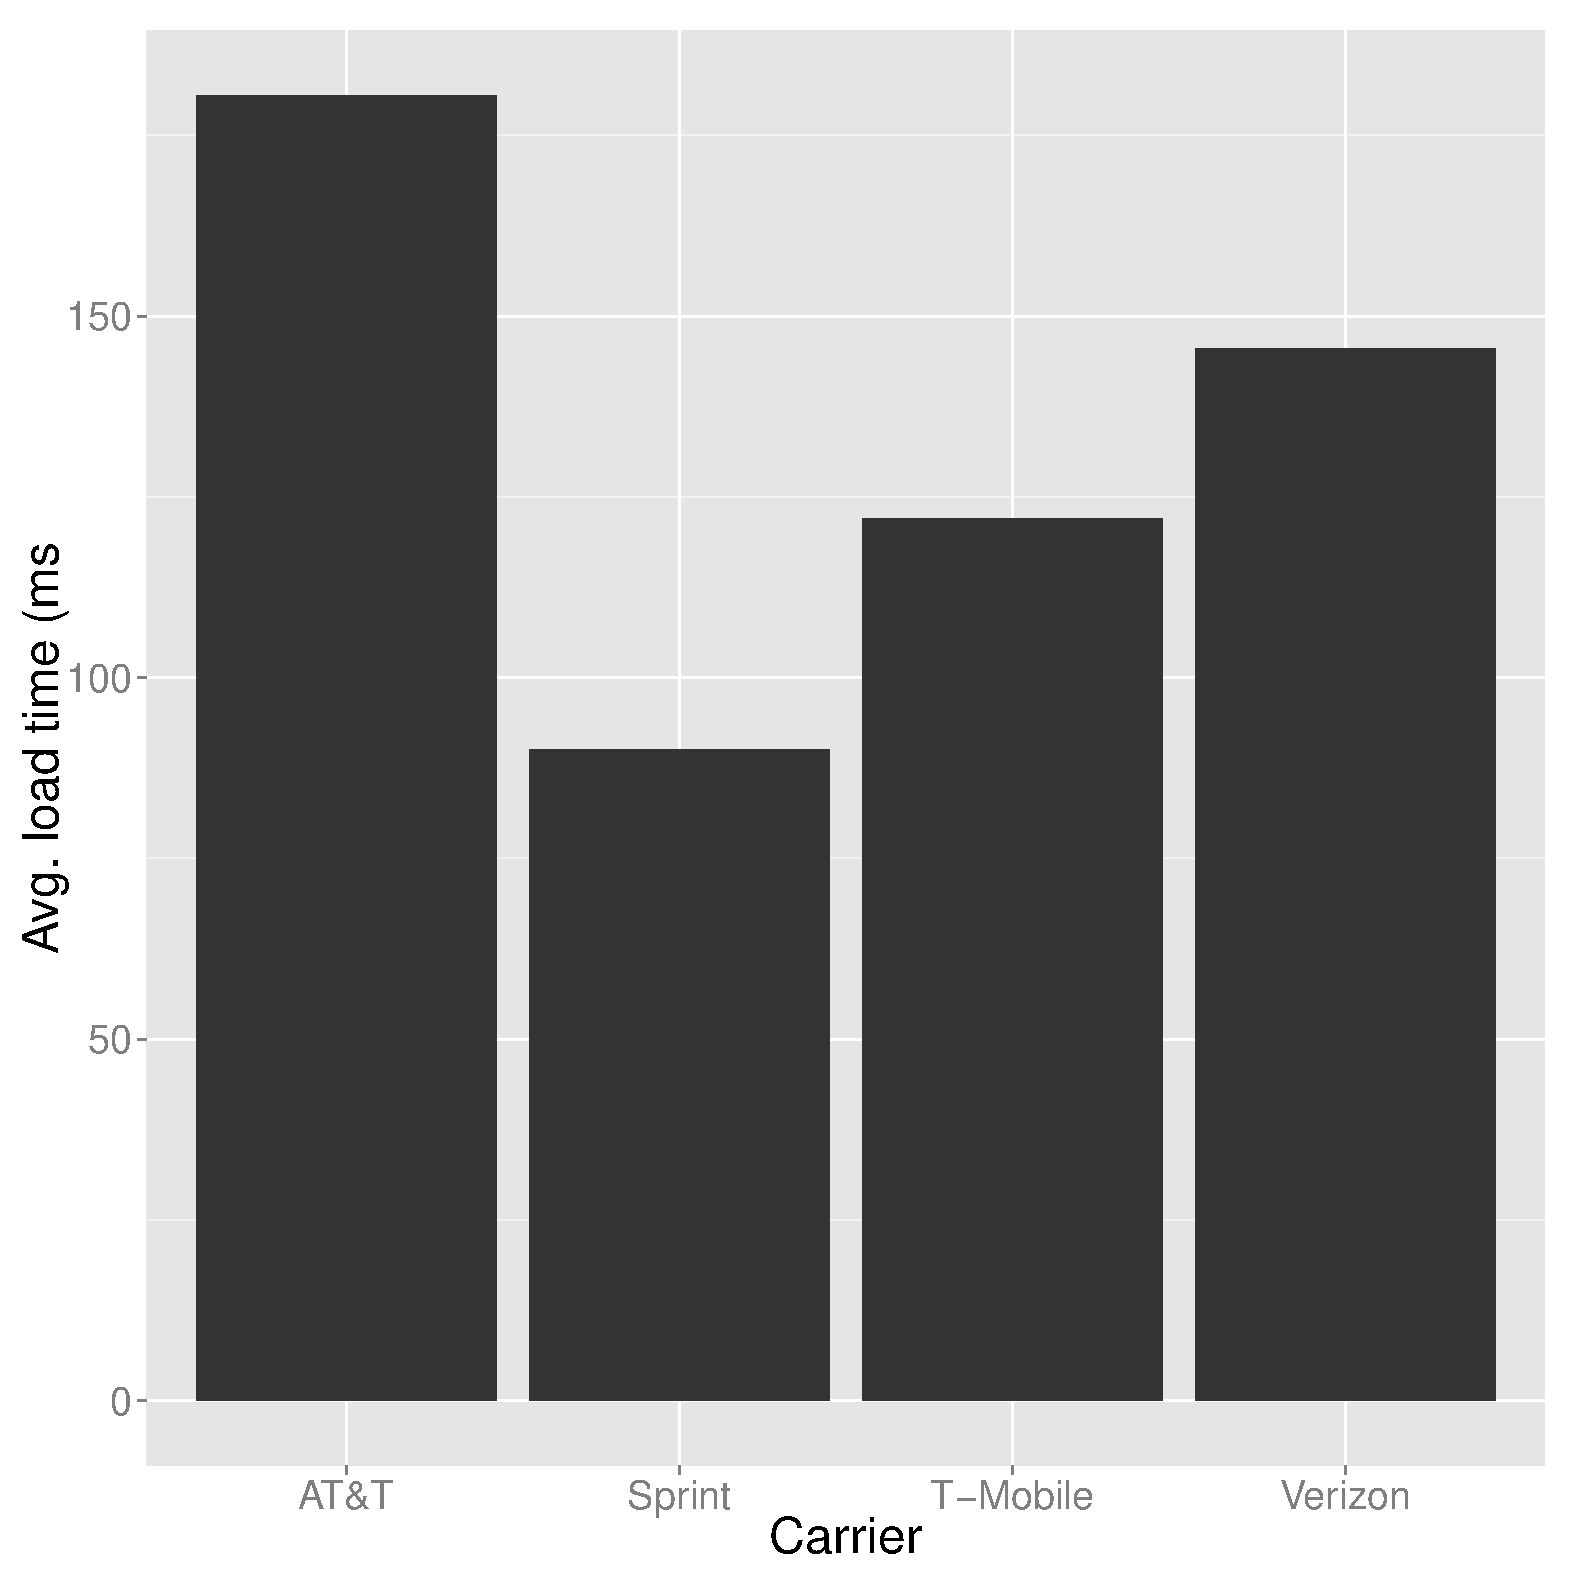
\includegraphics[width=4cm] {Images/dist1.pdf}}
		\caption{Visualization: Average \\ Load Times by Carrier
		 for App-A}
		\label{fig:staplerX}
	\end{subfigure}
	
	\centering
	\begin{subfigure}{0.49\linewidth}
		{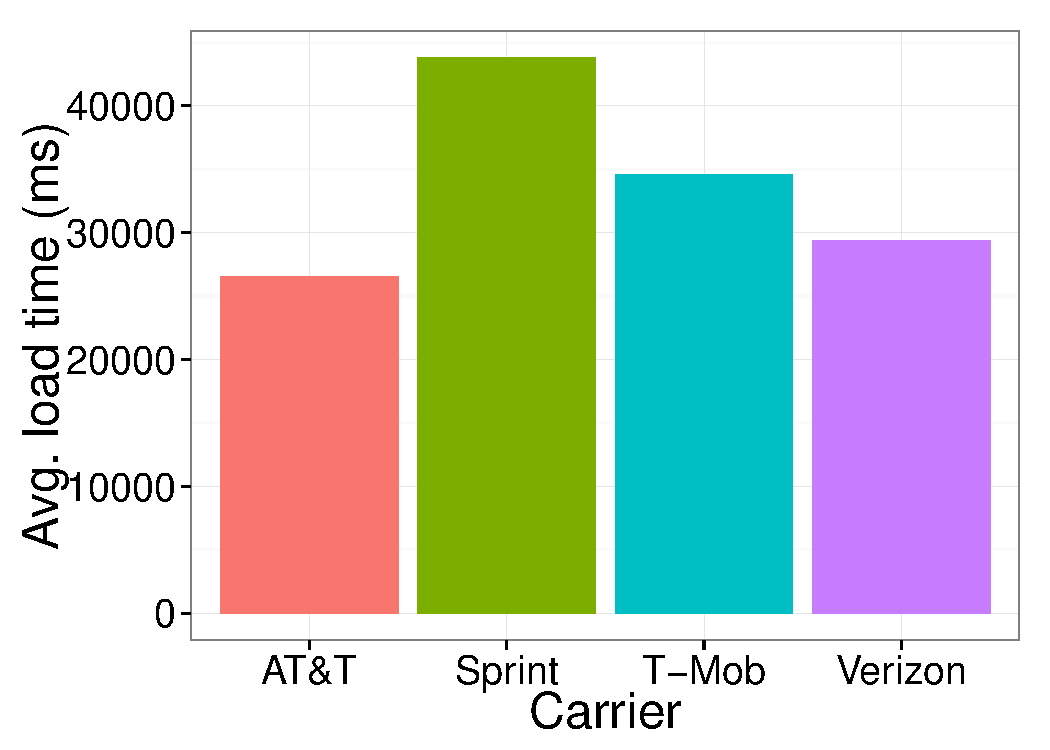
\includegraphics[width=4cm] {Images/dist2.pdf}}
		\caption{Scenario A: Average Load Times by Carrier}
		\label{fig:staplerX-a}
	\end{subfigure}
	\begin{subfigure}{0.49\linewidth}
		\centering
		{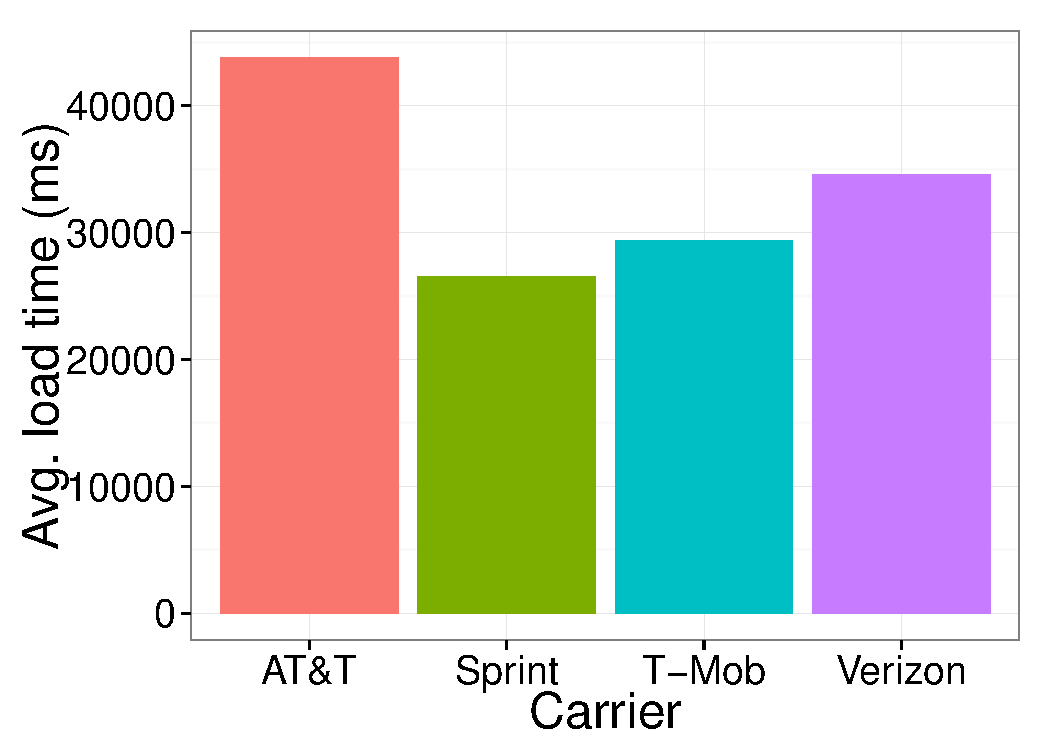
\includegraphics[width=4cm] {Images/dist3.pdf}}
		\caption{Scenario B: Average Load Times by Carrier}
		\label{fig:baseline_views}
	\end{subfigure}
	\caption{}
	\label{fig:staplerX-b}
\end{figure}

% \begin{figure}
% \vspace{-10pt}
% \CenterFloatBoxes
% \begin{floatrow}
% \ttabbox{%
%   \small
%   \begin{tabular}{cc} \hline
%   Carrier & Load Times (ms) \\ \hline
%   AT\&T & 180.55 \\ \hline
%   Verizon &  145.50\\ \hline
%   T-Mobile & 122.00 \\ \hline
%   Metro & 90.13 \\ \hline
%   \end{tabular}
% }{%
%   \caption{Data: Average Load Times by Carrier for App-A}\label{tab:staplerX}%
% }
% \killfloatstyle
% \ffigbox{%
%   \hbox{\resizebox{2cm}{2cm}{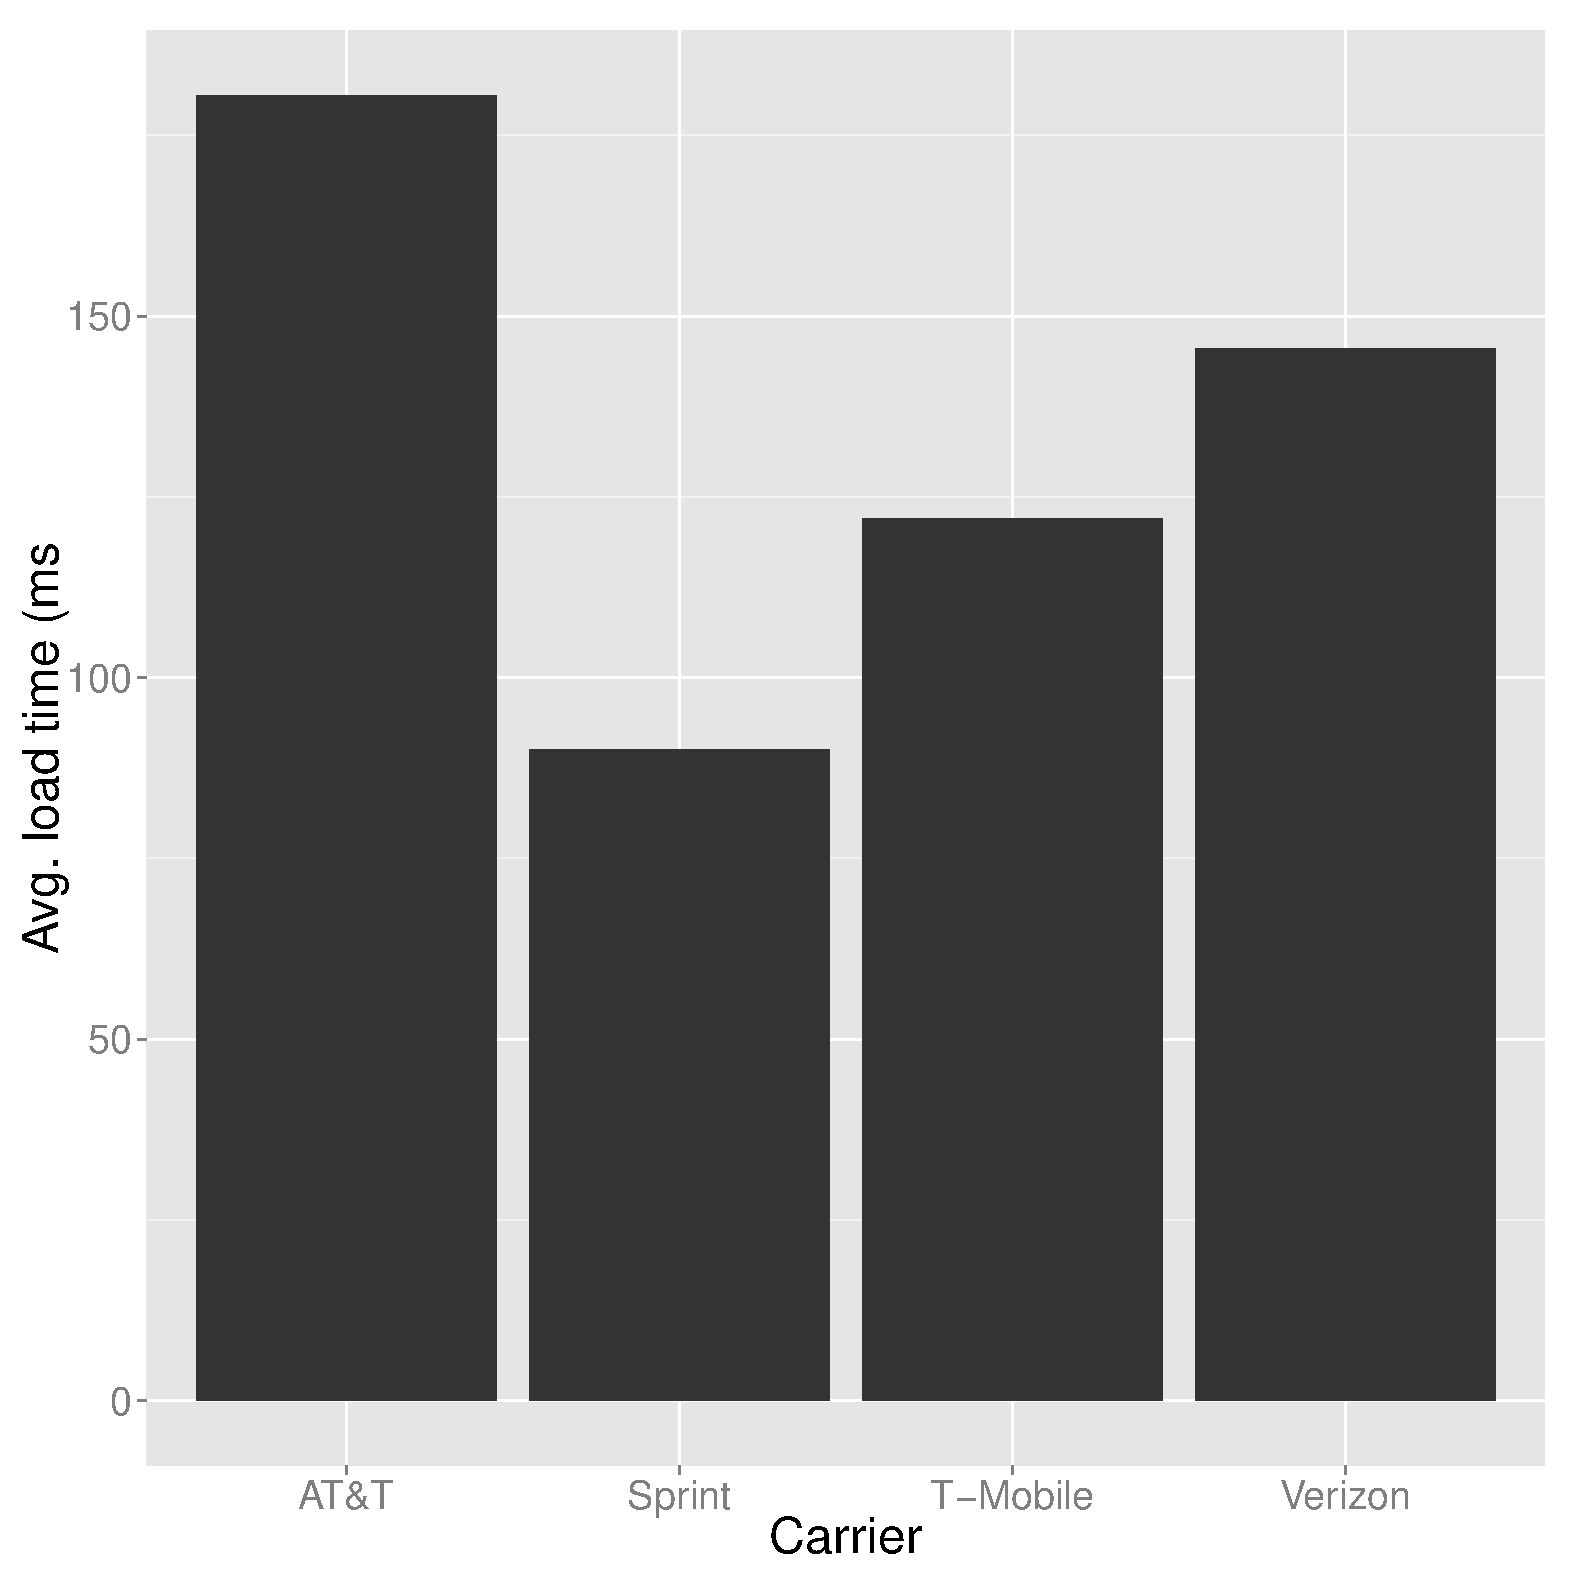
\includegraphics{Images/dist1.pdf}}}
% 
% }{%
%   \caption{Visualization: Average \\ Load Times by Carrier
%   for App-A}\label{fig:staplerX}%
% }
% \end{floatrow}
% \end{figure}
% 
% \begin{figure}
% \CenterFloatBoxes
% \begin{floatrow}
% \centering
% \ffigbox{%
%   \hbox{\resizebox{2cm}{2cm}{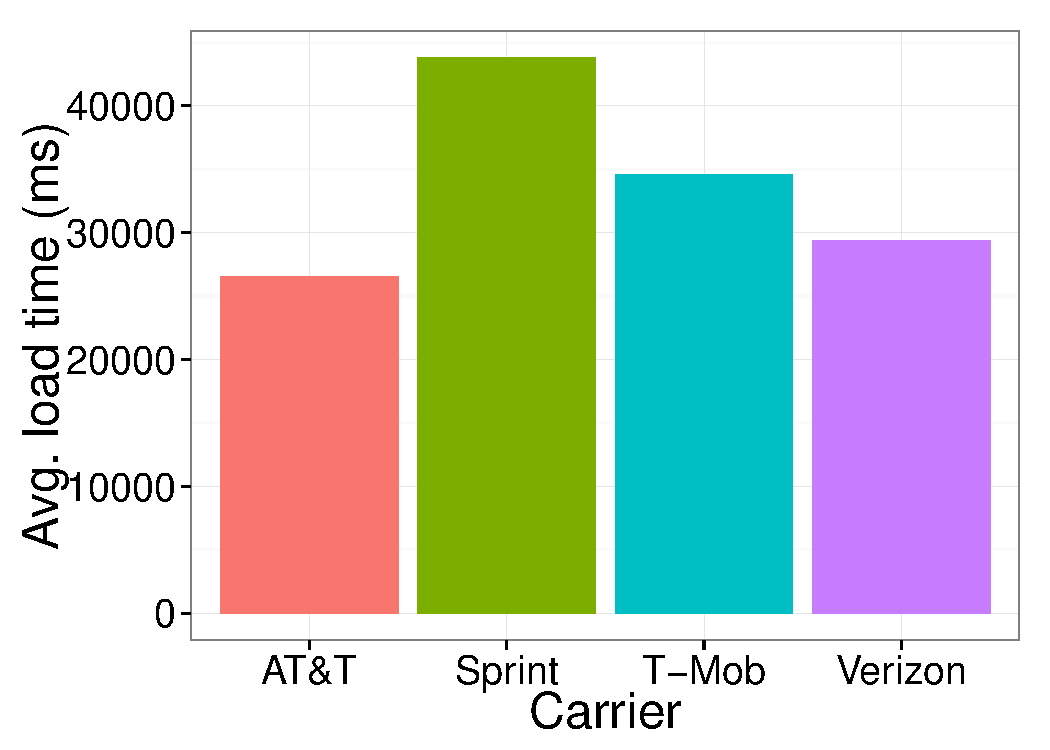
\includegraphics{Images/dist2.pdf}}}
% 
% }{%
%   \caption{Scenario A: Average Load Times by Carrier}\label{fig:staplerX-a}%
% }
% \killfloatstyle
% \ffigbox{%
%   \hbox{\resizebox{2cm}{2cm}{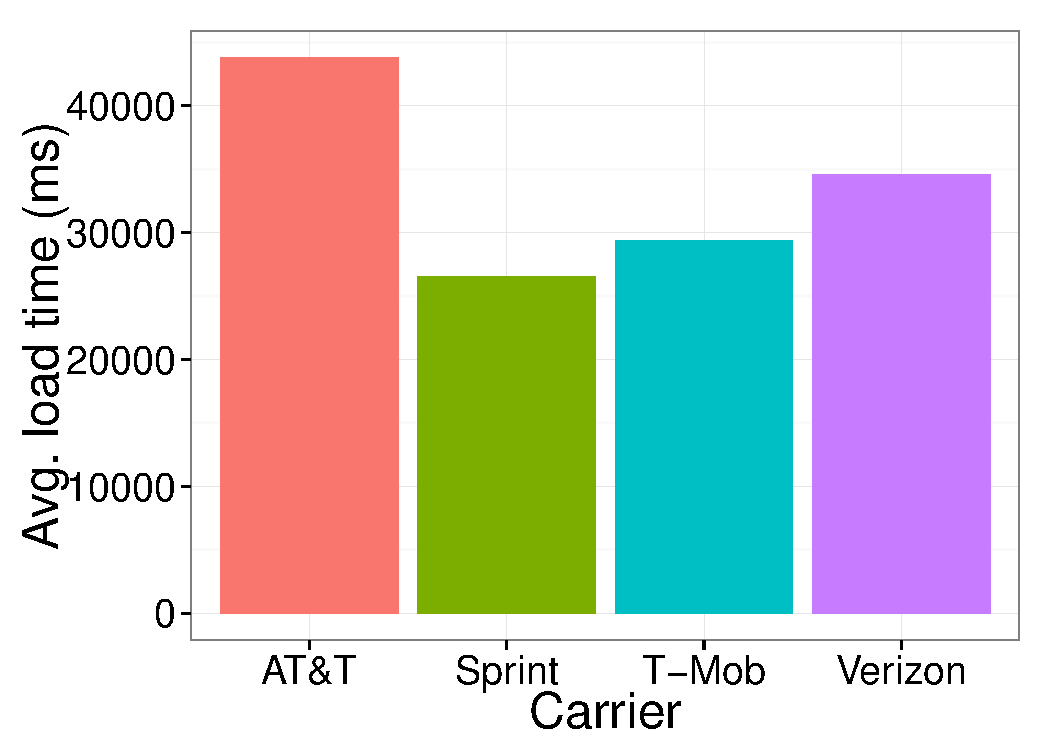
\includegraphics{Images/dist3.pdf}}}
% 
% }{%
%   \caption{Scenario B: Average Load Times by Carrier \srm{These figures seem to be for stores
% and stapers}}\label{fig:staplerX-b}%
% }
% \end{floatrow}
% \vspace{-12pt}
% \end{figure}



To explore the app behavior from different perspectives, the analyst generates
a large number of queries (and visualizations) of the form described above.
(3) The analyst then manually examines each result and decides
which ones are ``interesting''. This is a critical and time-consuming step.
Naturally, what makes a result interesting depends on the 
problem the analyst is trying to solve and the
attributes being compared.
For instance, the visualization of load times by carrier, as shown in Figure
\ref{fig:staplerX}, may be interesting if the overall load times for all
apps showed the {\it opposite} trend (e.g. Figure \ref{fig:staplerX-a}).
However, the same visualization may be uninteresting if the load times of all apps
follow a similar trend (Figure \ref{fig:staplerX-b}).
Thus, we posit that  a visualization is {\em potentially ``interesting'' if it shows 
a trend in the subset of data selected by the analyst
(i.e., metrics about App-A)
that deviates from the equivalent trend in the overall dataset (i.e., metrics
about all apps)}.
Of course, the analyst must decide if this deviation 
is truly an insight for this application.
(4) Once the analyst has identified interesting attributes and dimensions to query
against, the analyst may
then either share these result with others, further interact with
the displayed results (e.g., by drilling down or rolling up), or
start afresh with a new query.


Of the four steps in the workflow described above, the 
ones that are especially repetitive and tedious are steps (2) and (3)
where the analyst generates a large number of candidate aggregate queries, 
and examines each
of them in turn through visualization.
The goal of our system, \VizRecDB, is to automate these
labor-intensive steps of the workflow. 
Given a query $Q$ indicating the subset
of data that the analyst is interested in, \VizRecDB\ automatically {\em
identifies and highlights to the analyst the most interesting queries to ask using methods based on
deviation} (we formalize our notion of ``interestingness'' in Section~\ref{sec:problem_statement}).
Specifically, \VizRecDB\ explores the space of all possible {\it views} and
measures how much each view deviates from the corresponding view on the
entire underlying dataset (e.g. Figure~\ref{fig:staplerX} vs.
Figures~\ref{fig:staplerX-a} or \ref{fig:staplerX-b}.) 
By {\it view} we mean a (possibly multidimensional) GROUP BY/aggregate with one or more
measure attributes.
By generating and
scoring such views automatically, \VizRecDB\ effectively eliminates
steps (2) and (3) that the analyst currently performs. 
Instead, once \VizRecDB\
recommends interesting views, the analyst can evaluate this small
subset of views using domain knowledge and limit further
exploration to these views.  

The above example illustrates one particular use case for \VizRecDB,
particularly one where an analyst compares a subset of the data against all
the underlying data.
There are three use cases of \VizRecDB\ that are generalizations of the above
model and are supported by \VizRecDB:
\squishlist
  \item {\it Use Case I: Comparison of a subset of data against the entire
  underlying data}.
  This is the smartphone app metrics use case discussed above.
  \item {\it Use Case II: Comparison of a subset of data against all the
  remaining data}.
  Imagine that a medical researcher is studying a medical records dataset and
  wants to compare the set of patients with high medical expenses vs. 
  other patients. The techniques from the first use case can be used
  directly for this use case too.
  \item {\it Use Case III: Comparison of two distinct datasets}. Finally,
  imagine that in the app metrics example, an analyst would like to compare
  the metrics for two apps, say one app in the social category and another in
  the music category. In this case, the analyst will select the datasets
  by executing two different queries and \VizRecDB\ can be used to find
  interesting differences between the two datasets.
\squishend

In the rest of the paper, we center our discussion around Use Case I, however,
all our techniques apply unchanged to Use Cases II and III.

% \subsection*{Example 2: Medical Data}
% Next, let us examine a use case in a completely different problem domain that
% also involves analyses similar to Example 1, and therefore, can benefit from the
% automatic construction of interesting views of a user query.
% 
% Consider a medical researcher studying the cost of care for cancer
% patients\footnote{Real use scenario at an area hospital}. The goal of the study
% is to identify patients whose cost of care is significantly greater than
% average and try to explain the high cost of care. Potential reasons for
% high cost include treatments for late-stage cancers, old age of the
% population, longer survival time (chemotherapy for a longer duration), type of
% treatment etc.
% Note that the goal is {\it not} to build a predictive model for cost; rather, it
% is to perform exploratory analysis to explain {\it why} certain patients have
% high cost of care.
% As a first pass, assume that the researcher identifies high cost patients as those with
% cost that is greater than two standard deviations away from the average
% cost. This can be expressed via the following SQL query, assuming a table of
% patients with their treatment costs and other treatment-related information.
% \begin{align*}
% & \tt Q2\ = SELECT \ \ *\ FROM \ \ Patients \ \ where\ cost - \\
%   \ \ & \tt (SELECT\ AVG(cost)\ FROM\ Patients)\ >\\
%   \ \ & \tt 2\ *\ (SELECT\ STDDEV(cost)\ FROM\ Patients)
% \end{align*}
% 
% Once these patients have been identified, the researcher can begin to analyze
% the data to find potential reasons for their high cost of care (This is similar
% to Step 1 in Example 1).
% One technique to find potential reasons for high cost is to compare the
% high-cost population of patients to the remaining set of patients (called
% ``low-cost'' population).
% Similar to Example 1 above, we posit that the {\it characteristics that
% explain high cost are precisely those characteristics that are different between
% the high-cost and low-cost population}. 
% For instance, if the majority of
% high-cost patients were those with late-stage disease (sicker patients) while
% the low-cost patients were not, the researcher could reason that the sicker
% patients needed more medications or procedures, leading
% to higher cost overall. 
% Note that this analysis is similar to Example 1 where we
% compared the ``total sales by year'' for $Laserwave$ $oven$ vs. all store
% products.
% In this setup, we want to compare the ``total patients by disease stage'' for
% high-cost patients vs. low-cost patients. The only change in the problem
% formulation is that we are now comparing views of query Q2 against views of the
% remaining table, instead of views over the entire table. The rest of the
% framework remains unchanged. Therefore, \VizRecDB\ can be used to automatically
% construct a large number of views of the high-cost population, compare
% each view to the corresponding view over the low-cost population, and
% identify views showing the highest difference between the two populations. These
% views identify potential causes for high cost. Once the researcher has identified views of interest, he or she
% can follow up with more complex analyses like statistical significance testing or machine
% learning.
% 
% \subsection*{Example 3: Product Analysis}
% 
% Consider a company like Facebook\footnote{www.facebook.com} that continuously
% deploys changes to its website and mobile apps, and tracks user interaction
% through detailed logging. Product specialists at Facebook use these logs to
% study how different Facebook users respond to changes to the web or mobile
% experience \cite{DBLP:conf/vldb/AbrahamABB13}. Each user can be characterized by a large number
% of features such as location, age, device used, number of friends etc.
% For each user, the logs note the actions taken on the website or app such
% as likes, shares, comments, page visits etc. For example, in order to study
% the user response to an update to the mobile app, the specialist compares user
% interaction metrics for a large number of mobile users before and after the
% update (usually a week on week comparison). The goal is to find patterns in the
% interaction metrics based on different user characteristics. Therefore, if it
% appears that the average number of app visits on the iOS app have reduced
% signficantly following the update, it would indicate a problem with the iOS app.
% 
% In terms of the \VizRecDB\ framework, log data from the week following the app
% update constitutes the query results we seek to analyze and the log data from
% the prior week comprises the comparison dataset. As in Examples 1 and 2, the
% analysis process requires the specialist to create diverse views of the query
% results, compare views to equivalent views on the comparison dataset, and
% pick the views showing the highest difference. 
% \VizRecDB\ can therefore be used to automate this process and surface only the most
% interesting views.


\subsection*{Challenges and Contributions}

We previously described some of the vision for  \VizRecDB\ in our (4 page)
vision paper~\cite{DBLP:conf/vldb/Parameswaran2013}---that paper described the
challenges at a high level without any real implementation; in this paper, we
demonstrate that we can build real systems that efficiently search for the most
interesting views at interactive time scales.
% Efficiently and accurately producing the set of most interesting
% views (aggregate queries) for any dataset is challenging for several reasons:
% (1) We must determine metrics that accurately measure the ``deviation'' of a
% view with respect to the equivalent view on the entire database (e.g.,
% Figure~\ref{fig:staplerX} vs.~\ref{fig:staplerX-a}); 
% (2)  The space of candidate views grows as the square of the number of
% attributes, so we must intelligently explore the space of candidate views
% to support real time responses;
% (3) While executing queries corresponding to different views, we must share
% computation as much as possible. 
% For example, 
% we can compute multiple views and measure their deviation 
% all together in one query. Independent execution,
% on the other hand, will be expensive and wasteful;
% Queries to compute views and their
% deviation are highly similar and therefore
% independent execution is expensive and wasteful; 
% (4) We must prune low-utility views early on to avoid wasting resources and
% computation on these views; 
% (5) Since analysis must happen in interactive time scales, we must trade-off
% accuracy of visualizations or estimation of ``interestingness'' for reduced latency.

% in this paper, we demonstrate that we can build real systems that efficiently search for the most 
% interesting views, formalize the notion of ``interestingness'', and thoroughly
% explore the space of possible optimizations.
%In this work, we explored two distinct implementations of \VizRecDB, both on top
%of a database.
In this paper, we describe two implementations of \VizRecDB\ that address the
challenges from \cite{DBLP:conf/vldb/Parameswaran2013}.
In our first implementation, we implement \VizRecDB\ as a wrapper on top of a
database system and study how far we can push existing systems to support a
\VizRecDB-type workload.
In the second, we overcome the constraints of the DBMS API by writing a custom system
that  shares sequential scans and query results between views and employs statistical methods to 
perform aggressive pruning
based on intermediate results.
For each implementation of \VizRecDB, we also develop implementation-specific
optimizations that leverage the underlying system architecture.
% SRM already said
%At its core, given a query $Q$ indicating the subset of data that the analyst is
%interested in, the goal of \VizRecDB\ automatically {\em identifies and
%highlights to the analyst the most interesting views of the query results using
%methods based on deviation}.

The contributions of this paper are:
\squishlist
  \item We
  explore and evaluate two distinct implementations of the system, one as a
  wrapper around a database and another a custom solution.
  \item For the DBMS-backed implementation of \VizRecDB, we
  design a suite of optimizations to minimize the number of queries executed and to
  maximize the sharing of scans between queries (Section~\ref{XXX}).
  \item For the custom implementation of \VizRecDB, we cast the problem of
  finding the best views as a variant of both top-k ranking and the
  multi-armed bandit problem. We adapt heuristics from both problem spaces to
  perform aggressive pruning of views (Section~\ref{XXX}).
  \item We explore view pruning techniques based on data distribution
  to prune views even before they are evaluated by the \VizRecDB\ system 
  (Section~\ref{XXX}).
  \item We evaluate the performance of our optimizations on a range of
  real and synthetic datasets and demonstrate the resulting XXX speedup 
  (Section~\ref{sec:experiments}). We also demonstrate that our heuristics
  improve performance without affecting system accuracy.
\squishend

Finally, we note that although we are primarily motivated by efficiently 
identifying interesting views for the purposes of producing visualizations, 
the problem of finding aggregates of a dataset that display more (or less) variation
than other aggregates is broadly applicable in settings beyond visualization, including
outlier detection (finding outlier groups), data cleaning (finding erroneous 
data), feature selection (finding attributes with the most variability), and 
many others.



% of Step 1), we demonstrate that we can automatically explore various views of
% that data, evaluate each one for ``interesting''-ness and only surface the most
% promising views to the analyst. 



% In this demo, we demonstrate a system called \VizRecDB\
% \cite{DBLP:conf/vldb/Parameswaran2013} that automates the labor-intensive parts
% of the aforementioned data analysis process by automatically identifying and
% producing high-quality views for any input query. Specifically, given a query
% $Q$ posed by the user, \VizRecDB\ explores all possible views of $Q$, determines
% the ``interesting''-ness of each of the views based on deviation and returns to
% the user the set of views that it deems the most interesting. The user can then
% limit his analysis to this high-quality set of views.

% In the process of automatically producing an interesting set of views for any
% query, \VizRecDB\ must address a few challenges: (a) the size of the space of
% potential views increases as the square of the number of attributes in a table,
% and even for a moderately sized table (e.g. 1M rows, 100 attributes) generating
% all views is prohibitively expensive; as a result, \VizRecDB\ must intelligently
% explore this space; (b) computing each view and its utility independently is
% expensive and wasteful, and hence \VizRecDB\ must share computation between
% queries; and (c) since visual analysis must happen in real-time, \VizRecDB\ must
% tradeoff accuracy of views for reduced latency. In Section
% \ref{sec:system_architecture}, we describe how \VizRecDB\ addresses these
% challenges.


% Consider a medical researcher studying the cost of care for cancer patients. Her
% research involves the analysis of a set of 1M electronic medical records (EMRs).
% To analyze this data, the researcher identifies patients that cost
% significantly more than the average: specifically, she selects patients whose
% cost of care is greater than the average cost by two standard deviations. In
% terms of SQL, she runs the following query: \\

% \noindent 
% \begin{small}
% \begin{verbatim}
% Q = SELECT * FROM Patients where total_cost - 
% (SELECT AVG(total_cost) from Patients) as avg_cost
% > 2 * (SELECT STDDEV(total_cost) from Patients);
% \end{verbatim}
% \end{small}

% Once she has identified these patients, she must study various aspects of their
% care to determine the reason why the patients have large cost of care. For
% instance, she may study length of treatment, survival rate, severity of disease
% etc. For each of these parameters, she is interested in determining how the
% group of patients with high cost of care are different from the overall group of
% patients. As a result, she may construct various views of the data that
% compare various metrics between the high cost patients and the overall patient
% population. For instance, she may compare the distribution of length of
% treatment for the two populations, the average severity of the disease
% etc. Since there are a large number of metrics that may be responsible for high
% cost of care, the analyst must construct, visualize and examine a large number
% of views to identify interesting trends. For more than 5 metrics, this process
% quickly becomes tedious and time-consuming. We can significantly simplify and
% speed up the analysis process if we can automate the creation and evaluation of
% views.




% Since \VizRecDB\ must rank views based on utility, accurately measuring 
% utility is cruicial. \VizRecDB\ is based on the principle
% that it is the {\bf deviations from expected behavior that make a view
% interesting}. For instance, in the above example, the researcher would be
% interested in the fact that high-cost patients actually visit a specific set of
% doctors compared to the entire patient population. Similarly, the researcher
% would be interested in knowing that the high-cost patients have longer hospital
% stays compared to the rest of the population. Thus, given a query, interesting
% trends are those that differ significantly between the query and the underlying
% dataset. \VizRecDB\ therefore assigns higher utility to views that show divergent
% trends. (Since it may be more appropriate to compare the high-cost patients with
% other patients having the same disease but lower cost, so \VizRecDB\ allows the
% user to specify what dataset to compare with).



% \noindent There are several technical challenges that need to be addressed:
% 
% \begin{denselist}
% 
% \item For a given query, $n$, the total number of discriminating views, (even if
% we restrict ourselves to views that append a group-by and an aggregation) is
% likely to be very large to explore exhaustively and precisely. Generating each
% of $R_1(Q(D)),$  $\ldots,$ $R_n(Q(D))$, scoring them on utility, and then
% picking the best one is certainly not feasible for most databases. Thus, we need
% mechanisms to prune the space of views and compute their utility approximately.
% 
% \item Generating and scoring the discriminating views $R_i(Q(D))$ one-by-one may
% miss interesting optimization opportunities: First, we may share computation
% between discriminating views.  For example, the results of two views with
% different aggregates but the same group-by may be computed together in one
% query, followed by projecting out to reveal the two individual views.  Second,
% by evaluating the discriminating views in a deliberate order, we may be able to
% prune views with low utility (without evaluation) that are definitely not going
% to be recommended to the analyst.
% 
% \item Since visualizations tend to convey approximate information, e.g., a trend
% in a line plot may be more important than knowing the exact coordinates of each
% point, we can introduce approximations as part of \VizRecDB.  Thus, the utility of
% a discriminating view may be computed approximately but efficiently, and the
% recommended discriminating views can be populated with approximate results,
% based on synopses of the base data or of the query result, that can be generated
% much more efficiently.
% 
% \end{denselist}
